\documentclass{article}
\usepackage{enumitem}
\usepackage{indentfirst}
\usepackage{listings}
\usepackage{graphicx}
\usepackage{caption}
\usepackage{hyperref}
\usepackage{cleveref}
\usepackage[sorting=none]{biblatex}
\usepackage[a4paper,portrait,margin=1in]{geometry}

\addbibresource{writing.bib}
\hypersetup{
    colorlinks=true,
    urlcolor=blue,
    linkcolor=black,
    citecolor=cyan,
}
\title{ThemeChanger -- An Unified Theme Management Solution for Linux}
\author{Ioan Alexandru Popa}
\begin{document}
\maketitle

\begin{center}
    \url{https://github.com/ALEX11BR/ThemeChanger}
\end{center}

\begin{abstract}
    Changing the themes of desktop Linux applications is possible.
    Still, this process isn't the most straightforward one, as it involves modifying settings in multiple places, for every graphical library that supports theming.
    Also, the GNOME desktop environment has measures that prevent the easy customization of their applications' theme.
    In this paper, we propose an application that allows the user to more easily and consistently customize their Linux desktop applications, including GNOME's ones.
\end{abstract}

\section{Introduction}
In Linux, GUI (graphical user interface) applications have looks that can be configured.
Multiple GUI libraries for Linux exist, Qt and GTK being the most commonly used\cite{popcon}.
The libraries support user themes that change the way widgets (e.g. buttons, checkboxes) look like.
Themes can be downloaded from websites such as \url{https://www.gnome-look.org}.

All the Linux desktop environments have their core applications built with one library, but still have the possibility to run applications built with any other library.
While desktop environments provide their programs to change application themes, they often don't fully configure the other libraries' settings.

GTK~2 is used by the LXDE desktop environment and a couple applications like GIMP.
It has its specific format\cite{gtk2guide} for making themes.

GTK~3 is used by many desktop environments (e.g. Mate, XFCE) and applications (e.g. Inkscape).
Its themes are made in CSS (Cascading Style Sheets) format.

GTK~4 is used by the GNOME desktop environment and its applications.
Its themes are in a similar format to the one of GTK~3.
GNOME applications also use libadwaita, which gives them a specific look and feel that cannot be changed by regular means.

Qt is used by a couple of desktop environments (e.g. KDE Plasma) and many applications (e.g. VLC, Wireshark).
Unlike the GTK libraries that have some specific themes specified in a textual format that can be selected from, Qt's themes are handled by theme engines --- dynamic libraries that can draw the application widgets, and may leverage system-specific GUI libraries (in particular on Windows and macOS).
While a theme engine that uses the GTK 2 library\cite{qt5gtk2}, and thus its themes exists, it is seldomly used\cite{popcon}.
Kvantum is another theme engine for Qt (starting with version 5), with its user settable themes made using SVG (Scalable Vector Graphics --- a text format for specifying vector graphics).

Besides widget themes, there are also icon themes that have a common specification across GUI libraries.
Also, the aforementioned GUI libraries have a couple of other configurable parameters, such as fonts or whether buttons have icons or not.

\begin{figure}[h]
    \centering
    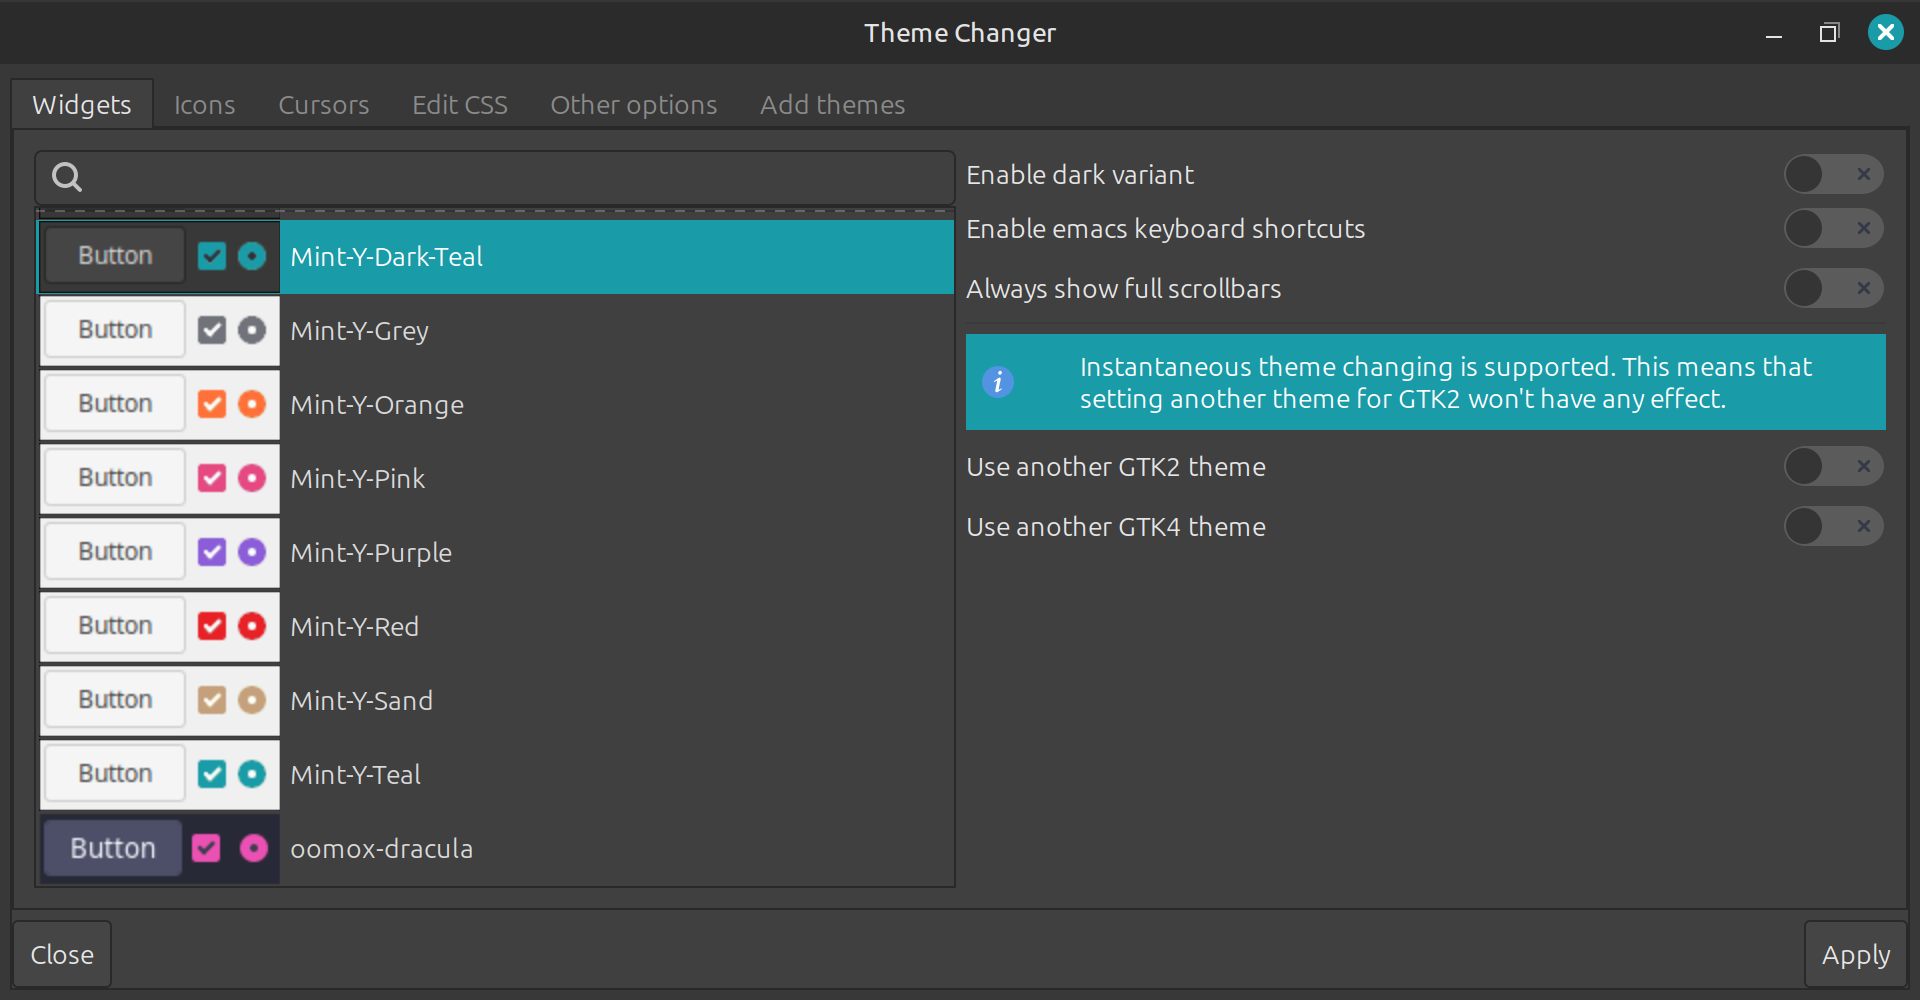
\includegraphics[width=0.75\textwidth]{screenshot1.png}
    \caption{Screenshot of ThemeChanger}
    \label{fig:screenshot1}
\end{figure}

ThemeChanger, as shown in \cref{fig:screenshot1}, is an application for Linux, for all its desktop environments, which enables the user to change the themes of GUI applications.
ThemeChanger is written in Python~3 using the GTK~3 library.

ThemeChanger lets the user change widget, icon, and mouse cursor themes, and also, to the extent they are supported by the GUI libraries, some options such as whether buttons or menus have icons or not.

ThemeChanger applies theme settings across all the GUI libraries that can be configured: GTK~2, GTK~3, GTK~4 (even for libadwaita applications), Qt (for the Kvantum theme engine).

\section{Live theme reloading}
Linux systems support the change of themes of GUI applications (only those based on GTK, starting with version 2) while they are running, using the XSETTINGS mechanism\cite{xsettings}.
Various theme settings can be set, including widget and theme names, antialiasing parameters, etc.
For the mechanism to work, the desktop environment will start a daemon which owns the theme values, and updates them when they are changed (by whatever mechanisms the desktop environment uses).
Besides desktop-environment-specific daemons, xsettingsd is a daemon meant for setups without desktop environments.

One of ThemeChanger's abilities is applying the themes to whichever one of the  desktop environment's mechanism is running.
To accomplish this, the function \verb|applyThemes| that sets the themes in the base configuration files is wrapped in the \verb|BaseApplyThemes| class, and various subclasses that inherit from \verb|BaseApplyThemes| add to that method the logic for setting the options in the desktop-environment-specific places.
When the app starts, depending on which daemons are running, an object of the according class gets instantiated, and whenever the user saves themes, the \verb|applyThemes| method of the aforementioned object gets called.

\section{GTK CSS Handling}
Starting from version 3, the GTK libraries' widget styles are specified using a custom implementation of CSS\cite{gtk3css}.
Among other things, GTK allows the user to specify their custom user CSS that overrides all themes and any other styles that an application may set for itself.

This means that even the libadwaita applications which impose their theme above the user selected themes can still have their looks customized by the user.
The styles of the libadwaita applications can be customized to any available third party theme by setting the user CSS of GTK~4 to have an universal CSS reset\footnote{The universal CSS reset clears all the style settings: \texttt{$*$ \{all: unset;\}}}, then an import of the theme.

\begin{figure}[h]
    \centering
    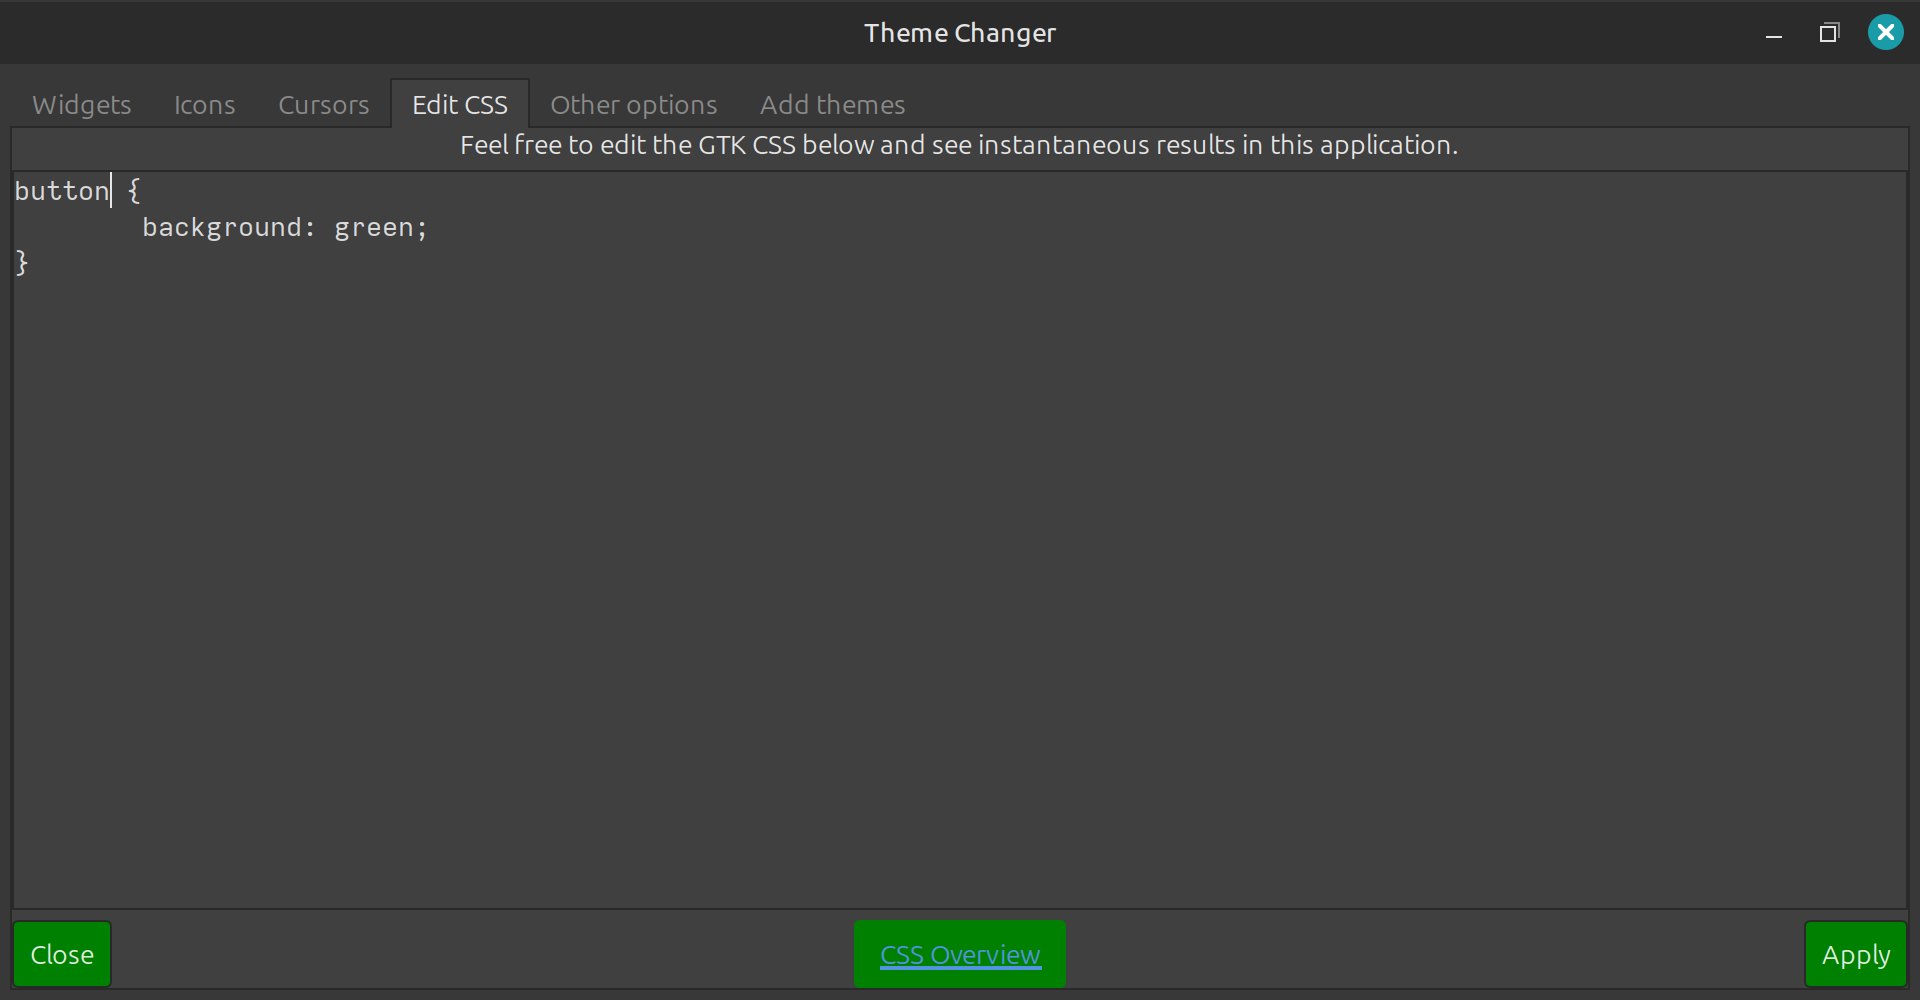
\includegraphics[width=0.75\textwidth]{screenshot2.png}
    \caption{ThemeChanger's GTK CSS editor}
    \label{fig:screenshot2}
\end{figure}

Another feature of ThemeChanger, as shown in \cref{fig:screenshot2}, is the user CSS editor that applies the changes to the ThemeChanger window as they are typed, and saves them to the user CSS on the save action.
If the typed user CSS were simply applied on top of the other CSS the application had loaded, this would not work on an edge case --- when the user CSS has a directive that gets removed in the editor, it would still be applied because the original user CSS that had the directive is still loaded and has effect.
To fix the aforementioned issue, we first apply an universal CSS reset, then apply the currently selected user theme, then we apply the CSS in the editor.

\section{Conclusions and Future Work}
We created an application that helps desktop Linux users configure uniformly from one place the GUI libraries' settings: themes, custom styles, fonts, etc.
We overcame the libadwaita barrier on third party themes so that GNOME users can change their applications themes like the other desktop environments' ones.

In the future we plan to implement a client for downloading third party themes from sources like \url{https://www.gnome-look.org}.
We also plan to implement some tricks to make Flatpak applications use themes that aren't installed on the running user's home folder.

\printbibliography
\end{document}
